\documentclass{article}
\usepackage{amsmath}
\usepackage{amssymb}
\usepackage[pdftex]{graphicx}
\usepackage[framed,numbered,autolinebreaks,useliterate]{mcode}
\lstset{breakatwhitespace=false}

\pdfpagewidth 8.5in
\pdfpageheight 11in
\topmargin -1in
\headheight 0in
\headsep 0in
\textheight 8.5in
\textwidth 6.5in
\oddsidemargin 0in
\evensidemargin 0in
\headheight 50pt
\headsep 0in
\footskip .75in

\title{STA 601 - Homework 9}
\author{Kedar Prabhudesai}
\date{October 11, 2013}

\begin{document}
\maketitle

\noindent {\Large\underline{\textbf{Hierarchical Model:}}} This model borrows information across experimental conditions. \\

Reaction times, $y_{ij},$ for subjects $j = 1,2,\ldots,n_i,$ in experimental conditions, $i = 1,2,\ldots,n.$\\

$y_{i} \sim Exp(\lambda_i)$, - Within Condition Model

$\lambda_i \sim Gamma(a,b).$ - Between Condition Model.\\

Priors on $a$ and $b.$

$a \sim e^{-a\alpha_a}$

$b \sim Gamma(\alpha_b,\beta_b).$\\

\noindent \underline{\textbf{Posterior Computation:}}\\
\begin{align*}
p(\lambda_1,\lambda_2,\ldots,\lambda_n,a,b \mid y_1,y_2,\ldots,y_n) &\propto p(y_1,y_2,\ldots,y_n \mid \lambda_1,\lambda_2,\ldots,\lambda_n,a,b) \times p(\lambda_1,\lambda_2,\ldots,\lambda_n \mid a,b) \times p(a) \times p(b)\\
&\propto \prod_{i=1}^{n}{\prod_{j=1}^{n_i}{p(y_{ij} \mid \lambda_i,a,b)}}\prod_{i=1}^{n}{p(\lambda_i \mid a,b)} \times p(a) \times p(b)
\end{align*}

\pagebreak

\noindent \underline{\textbf{Full Conditionals:}}\\
\begin{itemize}
\item $p(\lambda_i \mid a,b,y_1,y_2,\ldots,y_n)$
\begin{align*}
p(\lambda_i \mid a,b,y_1,y_2,\ldots,y_n) &\propto p(\lambda_i \mid a,b)\prod_{j=1}^{n_i}{p(y_j \mid \lambda_i,a,b)}\\
&\propto \lambda_i^{a-1}exp(-\lambda_ib) \prod_{j=1}^{n_i}{\lambda_iexp(-\lambda_iy_j)}\\
&\propto \lambda_i^{a-1}exp(-\lambda_ib) \lambda_i exp\left(-\lambda_i\sum_{j=1}^{n_i}{y_j}\right)\\
&\propto \lambda_i^{(a+n_i)-1}exp\left[-\lambda_i\left(b+\sum_{j=1}^{n_i}{y_j}\right)\right]\\
\therefore p(\lambda_i \mid a,b,y_1,y_2,\ldots,y_n) &\sim Gamma\left(a+n_i,b+\sum_{j=1}^{n_i}{y_j}\right).
\end{align*}

\item $p(a \mid \lambda_1,\lambda_2,\ldots,\lambda_n,b,y_1,y_2,\ldots,y_n)$
\begin{align*}
p(a \mid \lambda_1,\lambda_2,\ldots,\lambda_n,b,y_1,y_2,\ldots,y_n) &\propto p(a) \prod_{i=1}^{n}{p(\lambda_i \mid a,b)}\\
&\propto exp(-a\alpha_a)\prod_{i=1}^{n}{\lambda_i^{a-1}exp(-\lambda_ib)}\\
&\propto \left(\prod_{i=1}^{n}{\lambda_i}\right)^{a-1}exp(-a\alpha_a)
\end{align*}
We can sample from this distribution in Matlab by using `randsample' which is similar to `sample' in R.

\item $p(b \mid \lambda_1,\lambda_2,\ldots,\lambda_n,a,y_1,y_2,\ldots,y_n)$
\begin{align*}
p(b \mid \lambda_1,\lambda_2,\ldots,\lambda_n,a,y_1,y_2,\ldots,y_n) &\propto p(b) \prod_{i=1}^{n}{p(\lambda_i \mid a,b)}\\
&\propto b^{\alpha_b-1} exp(-b\beta_b) \prod_{i=1}^{n}{\lambda_i^{a-1}exp(-\lambda_ib)}\\
&\propto b^{\alpha_b-1} exp(-b\beta_b) exp\left(-\sum_{i=1}^{n}{\lambda_i}b\right)\\
&\propto b^{\alpha_b-1} exp\left[-b\left(\beta_b+\sum_{i=1}^{n}{\lambda_i}\right)\right]\\
\therefore p(b \mid \lambda_1,\lambda_2,\ldots,\lambda_n,a,y_1,y_2,\ldots,y_n) &\sim Gamma\left(\alpha_b,\beta_b+\sum_{i=1}^{n}{\lambda_i}\right).
\end{align*}
\end{itemize}

\pagebreak

\noindent \underline{\textbf{Gibbs Sampling:}}\\
Start with $\{a^{(0)},b^{(0)}\}$.
\begin{itemize}
\item Draw, $\lambda_i^{(s)} \sim Gamma\left(a^{(s)}+n_i,b^{(s)}+\sum_{j=1}^{n_i}{y_j}\right)$, i=1,2,\ldots,n.
\item Draw, $a^{(s+1)} \sim \left(\prod_{i=1}^{n}{\lambda_i^{(s)}}\right)^{a_{grid}-1}exp(-a_{grid}\alpha_a)$, using Griddy Gibbs (`randsample' in Matlab).
\item Draw, $b^{(s+1)} \sim Gamma\left(\alpha_b,\beta_b+\sum_{i=1}^{n}{\lambda_i^{(s)}}\right)$.
\item Repeat.
\end{itemize}

Given below are results. The dots in Magenta denote the true values of $\lambda_i$ used to simulate data. Blue lines denote means and $95\%$ Credible Intervals.\\

\begin{center}
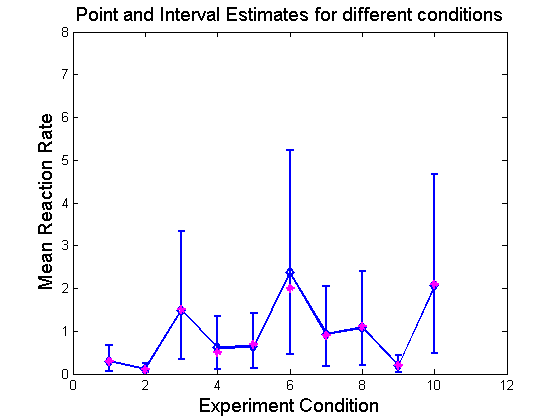
\includegraphics[scale=0.75]{HierarchicalModel.png}\\
\end{center}

\pagebreak

\noindent {\Large\underline{\textbf{Non-Hierarchical Model:}}} This model does NOT borrow information across experimental conditions. To achieve that, we group together data across experimental conditions and use a common model for the data. \\

Reaction times, $y_k,$ for subjects $k = 1,2,\ldots,m.$ Where, $m$ is the total number of data points pooled across all conditions.\\

$y \sim Exp(\lambda),$

$\lambda \sim Gamma(a,b).$

\noindent \underline{\textbf{Posterior:}}\\

\begin{align*}
p(\lambda \mid y) &\propto L(y;\lambda)p(\lambda)\\
&\propto \prod_{k=1}^{m}{\lambda}exp(-\lambda y_k) \lambda^{a-1} exp(-\lambda b)\\
&\propto \lambda^{a+m-1}exp\left[-\lambda\left(b+\sum_{k=1}^{m}y_k\right)\right]\\
p(\lambda \mid y) &\sim Gamma\left(a+m,b+\sum_{k=1}^{m}y_k\right)\\
\end{align*}

Therefore, the posterior mean is given by, $E(\lambda \mid y) = \frac{a+m}{b+\sum_{k=1}^{m}y_k}$
Using, $a = 2$, $b = 3$, (same initial values used for Gibbs Sampler), $m = 835$ we get, $E(\lambda \mid y) = 2.4191.$ If we plot this on the previous plot (red line), we can see that it is not a very good estimator for the condition specific reaction times.\\

\begin{center}
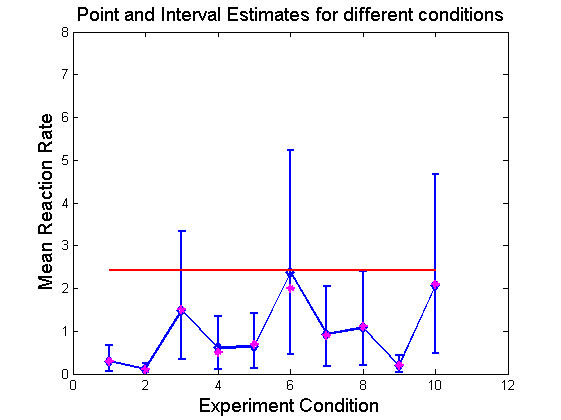
\includegraphics[scale=0.75]{NonHierarchicalModel.png}\\
\end{center}

\pagebreak
\noindent {\Large\underline{\textbf{Appendix:}}}\\
\lstinputlisting{C:/Users/ksp6/Documents/Classes/2013-Fall/STA601-BayesAndModStats/homeworks/hw9/hw9.m}

\end{document}